\section{experiments and results}
We study two important ecology phenomena, for each time period and location, 
wether there is snowfall and are there many plants with green leaves? We discuss the experimental setup 
and the results and evaluation below.
\subsection{Snow Case}
\subsubsection{Single Image Classification}
We are using the same hand-labeled dataset as in \fxnote{cite{workshop}}.
Beyond combining visual features, 
we build CNN visual model for our snow scene classification problem 
by fine-tuning Imagenet pre-trained model with the 8000 training images. The best 
performance in \fxnote{cite{workshop}} using visual features with SVM is $80.50\%$ acuracy.
On the same testing set of 2000 images, our CNN model achieves $88.06\%$ accuracy as a significant 
improvement. Details of comparison between performance of CNN model
 and other visual features are  are presented in table ~\ref{tab:snow}. Therefore, we use this as our recognitiion model for final predictions.

Figure ~\ref{fig:PR_ROC_snow} compares classification performance of CNN with 
individual visual features and their combination in terms of an ROC curve, 
as well as a precision-recall curve in which the task is to retrieve photos containing snow.
The precision-recall curve of CNN shows that at about $50\%$ recall, precision os very near to $100\%$, 
while even at $80\%$ recall, precision is still above $90\%$. This is a nice feature because 
in many applications, it may not be necessary to correctly 
classify all images, but instead it is important to find some images that most likely contain snowy 
scene.

We now turn to present experimental resutls for estimating geo-temporal distributions of snowfall.

\subsubsection{Snow Prediction on Cities}
To compare with existing results in \fxnote{cite{workshop}} using tag based method,
we first test how well our image-content based method can predict snowfall on daily base at a local scale, 
and in particular 
for the same four U.S. metropolitan areas, New York City, Boston, Chicago and Philadelphia. 
Table~\ref{tab:city_conf_tag_vision} 
shows some basic statistics for these 4 cities, and results of these classifiers. 
Best preformance obtained when we combine 
the confidence scores of tags and visual model based on CNN. For each of the method, 
Chicago gives the highest accuracy while Philadelphia gets the lowest accuracy. 
It's reasonable considering that Chicago has the most active Flickr users per
day (94.9) while Philadelphia has the least (43.7). 

There is not a clear evidence that visual evidence is more informative in estimating snowfall 
presence. In contrast, it gets lower accuracy in all these 4 cities. But combining tag and visual 
confidence achieves considerable improvement in performance. We apply this combined model 
in the following experiments.

\subsubsection{Continental-scale Snow Prediction}
Adding visual evidence, we reconstruct Satellite maps and 
evaluate our model in continental scale. We follow the same metric in \fxnote{cite{www}} to produce 
estimation at resolution of $1 \times 1$ degree (roughly $100 \times 100 km^2$) square and 1 map for 
every day in 2009 and 2010.

Figure ~\ref{fig:snowcurve} shows the precision and recall curve of snow prediction in 
continental-scale.
Here we limit our predictions for the bins which have photos taken at that 
time and location, we do this by keeping the bins have ground truth and photos at the same time. 
We computed our confidence scores based on tags and image-classification, then we trained 
simple decision tree to learn the correct thresholds to make final prediction. We achieve 
almost 0.5\% over the baseline (cutting the error rate by more than 20\%), the baseline in 
our case is the majority class which predicts now snow all the time. 



\begin{table}\centering
\caption{\textbf{Performance of different features for snow detection using SVMs for classification and compared with CNN model.}}
\label{tab:snow}
\begin{tabular}{@{}lcr@{}}\toprule
Feature & Kernel & Accuracy\\\midrule
Random Baseline & --- & 50.0\%\\
Gist & RBF & 73.7\%\\
Color  & $\chi^2$ & 74.1\%\\
Tiny & RBF & 74.3\%\\
Spatial Color Moments & RBF & 76.2\%\\
Spatial pyramid LBP & RBF &\textbf{77.0\%}\\\midrule
All features  & linear & \textbf{80.5\%}\\
CNN& -& \textbf{88.06\%}\\
\bottomrule\\
\end{tabular}
\end{table}


\begin{figure*}[th!]
\begin{center}
\vspace{-16pt}
\begin{tabular}{cc}
 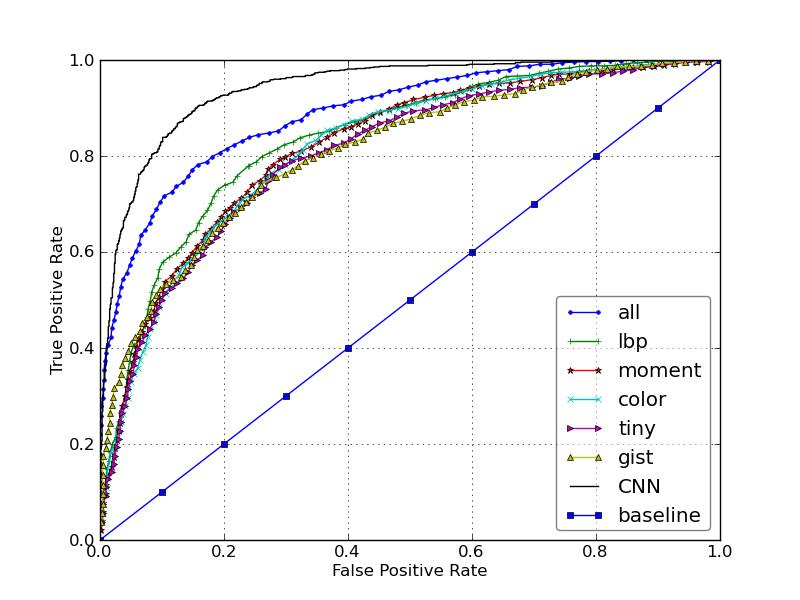
\includegraphics[width=0.4\textwidth]{figure/ROC-CNN-curves.jpg} &
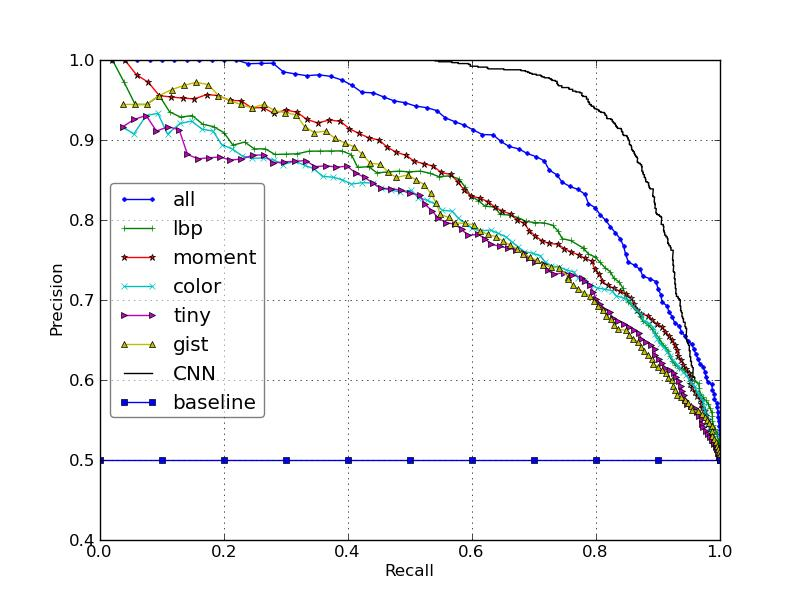
\includegraphics[width=0.4\textwidth]{figure/PR-CNN-curves.jpg} \\
\end{tabular}
\end{center}
\vspace{-8pt}
\caption{
Snow classification results for different features and combinations, in terms of {\textit{(left):}} ROC curves for the task of classifying snow vs. non-snow images; and 
{\textit{(right):}} Precision-Recall curves for the task of retrieving snow images.
}
\label{fig:PR_ROC_snow}
\end{figure*}


\begin{table*}\centering
\caption {\textbf{Selected basic statistics during 2007 to 2010 for the 4 cities and results of the likelihood model using tags and vision evidence.}}
\label{tab:city_conf_tag_vision} 
\begin{tabular}{@{}crrrrrr@{}}\toprule
City &  baseline & active user/day  & snow days &  tag confidence &  vision conf & tags conf and vision conf \\\midrule
{NYC} & 85.00\% & 65.6 & 185 &90.42\%&90.29\% &92.34\%\\
{Chicago} &72.80\% & 94.9 & 418 &94.12\% &93.16\% &95.08\%  \\
{Boston} & 75.60\%& 59.7 & 373 &89.18\%&85.21\% & 91.23\% \\
{Philly} & 80.50\% & 43.7 & 280 & 89.19\% &85.09\% & 89.19\%  \\
\bottomrule
\end{tabular}
\vspace{-12pt}
\end{table*}

\begin{figure*}
%{\small{
\begin{center}
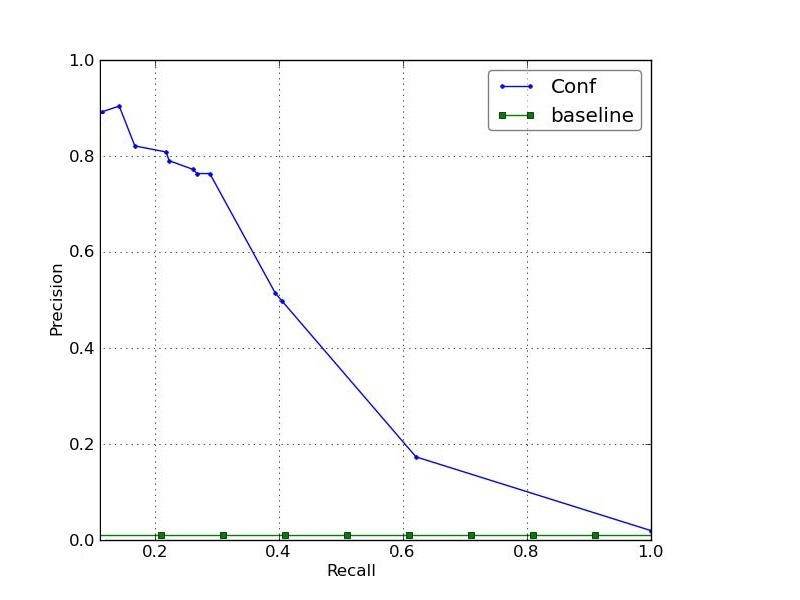
\includegraphics[width=0.40\textwidth,clip,trim=0.4in 0 0.8in 0]{figure/PR-snow.jpg}
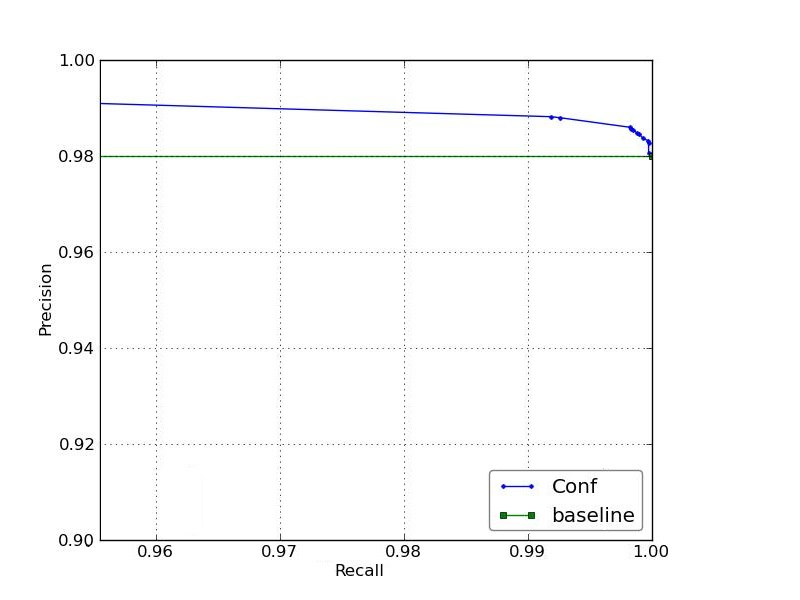
\includegraphics[width=0.40\textwidth,clip,trim=0.4in 0 0.8in 0]{figure/PR-nonsnow.jpg}
\end{center}
%}}
\vspace{-12pt}
\caption{Precision and recall curve of snow prediction (left) and nonsnow (right) in continental scale.}
\label{fig:snowcurve}
\vspace{-12pt}
\end{figure*}